%% ---------------------------------------------------------------------------
%% intro.tex
%%
%% Introduction
%%
%% $Id: intro.tex 1477 2010-07-28 21:34:43Z palvarado $
%% ---------------------------------------------------------------------------
\chapter{Introducción}
\label{chp:intro}

\section{Gestión actual de parqueos en el Campus Tecnológico Local San José}
En la sede universitaria del Instituto Tecnológico de Costa Rica (TEC) en San José, 
hay tres estacionamientos de automóviles, los cuales pueden ser usados ya sea por profesores,
estudiantes o visitantes temporales. De los tres estacionamientos, hay dos que pertenecen a la institución
y uno es alquilado. En el estacionamiento interno hay espacio para 12 vehículos y 5 motocicletas.
Debido a que es muy poco espacio, la institución compró la edificación Casa Pacheco, ubicada al costado norte
de la cuadra principal del Campus Tecnológico Local San José, sobre avenida 11, entre calles 5 y 7.
En Casa Pacheco hay espacio para 10 vehículos, y no hay espacio para motocicletas. A pesar de esta adquisición,
el espacio continuó siendo insuficiente, por lo que se decidió alquilar el estacionamiento City, ubicado al costado sur
de la cuadra principal del Campus Tecnológico Local San José, sobre calle 5. La Fig. \ref{fig:ubiacion_parqueos},
muestra la ubicación del Campus según Google Maps.
En cada uno de los estacionamientos hay un guarda que se encarga de la seguridad en el espacio.

\begin{table}[H]
	\centering
	\begin{tabular}{| c | c | c |}
		\hline
								& Automóviles & Motocicletas \\
		\hline
		Estacionamiento Interno & 12 		  & 5			 \\
		\hline
		Casa Pacheco			& 10		  & 0			 \\
		\hline
		Estacionamiento City	& 24		  & 2			 \\
		\hline
		Total					& 46		  & 7			 \\
		\hline
	\end{tabular}
	\caption{Número de espacios por estacionamiento.}
	\label{tab:numero_espacios}
\end{table}

\begin{figure}[H]
	\centering
	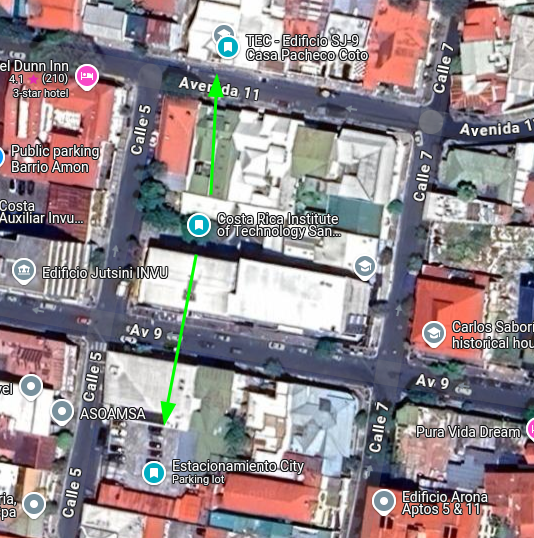
\includegraphics[width=0.8\textwidth]{fig/proy/ubiacion_parqueos.png}
	\caption{Ubicación de los parqueos obtenida mediante Google Maps.}
	\label{fig:ubiacion_parqueos}
\end{figure}

La entrada al estacionamiento interno se encuentra en el extremo opuesto de la entrada principal,
donde se encuentra ubicada la caseta del guarda de seguridad.
Para ingresar, los conductores deben primero detenerse frente a la caseta, notificar al guarda de seguridad
y luego rodear la cuadra hasta llegar al portón de acceso al parqueo.

Si no hay espacio disponible, se permite utilizar el estacionamiento de Casa Pacheco.
En ese caso, es necesario consultar con un guarda ubicado dentro del edificio si hay cupo.
Si la respuesta es afirmativa, el guarda de seguridad abre el portón manualmente para permitir
el ingreso del vehículo. Dado lo reducido del espacio, en algunas ocasiones el guarda debe asistir
a los conductores para maniobrar y estacionar adecuadamente.


Como última opción está el estacionamiento City. En cuanto a este estacionamiento,
también es necesario preguntar al personal de seguridad si hay espacios disponibles.
Si los hay, se abre el portón para que los vehículos puedan ingresar.


Cabe señalar que solo el portón del estacionamiento interno cuenta con un semáforo que indica si hay espacios disponibles.
Este semáforo es operado manualmente por los guardas de seguridad.

\begin{figure}[H]
	\centering
	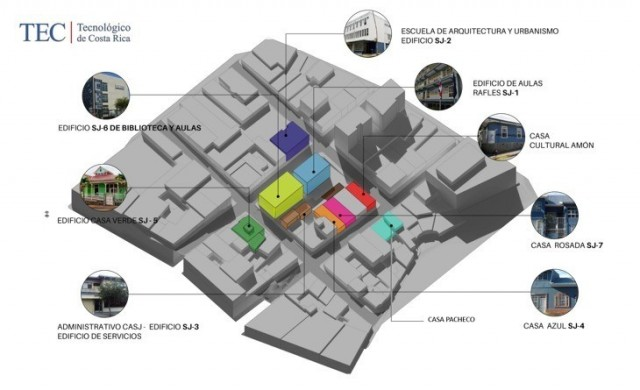
\includegraphics[width=0.8\textwidth]{fig/proy/croquis_del_campus_tec_san_jose.jpeg}
	\caption{Croquis del Campus Tecnológico Local San José \cite{tecCroquisSJ}.}
	\label{fig:croquis_tec}
\end{figure}

Actualmente, no existe una coordinación entre los distintos guardas para la gestión conjunta de los estacionamientos.
Además, las cámaras de seguridad instaladas en cada parqueo no pueden ser observadas por estos guardas,
ya que el monitoreo está a cargo de un grupo distinto ubicado en Casa Rosada,
dentro del campus principal (ver Figura \ref{fig:croquis_tec}).
Dicho grupo y los guardas de los parqueos operan de forma independiente, pues pertenecen a contratos diferentes.

El equipo de monitoreo en Casa Rosada tiene como responsabilidad principal la seguridad general del campus,
incluyendo la vigilancia ante robos y daños a la propiedad. Por su parte,
los guardas de los estacionamientos se encargan principalmente de controlar el ingreso de personas y vehículos.
Las horas de mayor uso del parqueo ocurren en las mañanas, entre las 7:00 a.m. y las 9:20 a.m.,
cuando se genera una leve congestión debido a la búsqueda de espacios disponibles.

\subsection{Reglamentos y logística}
Los automóviles que ingresan deben respetar un reglamento 
interno para garantizar la seguridad y el orden dentro del Campus.
Para tal propósito, al ingresar a la institución se debe registrar el número de placa y el nombre del usuario.
Adicionalmente, es aconsejable que los usuarios que ingresan estacionen sus vehículos
en lugares que no dificulten el ingreso o salida de nuevos vehículos cortando la visibilidad;
y así agilizar la movilidad dentro de estacionamiento y la búsqueda de estacionamiento.
En horas de alto flujo vehicular el registro y control de los vehículos que ingresan
genera cuellos de botella en la entrada del Campus, ralentizado el acceso y causando congestión.

\subsection{Factores tecnológicos}
En cada uno de los estacionamientos existe una cámara de seguridad. En el estacionamiento interno,
esta cámara está observando la entrada principal en una vista elevada, y también tiene una vista elevada del estacionamiento. 
En Casa Pacheco hay una única cámara que solo apunta a la entrada. Está en una pared al fondo y permite 
observar parcialmente la ubicación de los automóviles según lo reportado por el equipo de monitoreo.
Sin embargo, esta cámara por el momento está inactiva a espera de mantenimiento.
En el estacionamiento City hay un cámara con vista elevada desde la esquina suroeste. Da una vista desde arriba de todos
los automóviles en el estacionamiento. La institución solo tiene acceso a la
cámara del estacionamiento interno. A las cámaras de Casa Pacheco y Estacionamiento City solo tiene acceso 
monitoreo en Casa Rosada. Los guardas de seguridad de cada estacionamiento no tienen acceso a ninguna de las cámaras.

\section{Experiencias previas de control vehicular en el TEC}
En un primer intento por abordar la problemática de gestión vehicular,
el Campus Tecnológico Local San Carlos solicitó la implementación de un sistema de reconocimiento automático
de placas vehiculares (ANPR) como parte de un sistema más amplio de gestión inteligente de parqueos (IPLMS).
Este proyecto inicial buscaba aprovechar los recursos ya existentes en dicha sede, como las cámaras de seguridad,
con el objetivo de mejorar la coordinación y uso eficiente de los espacios de estacionamiento.

El diseño original logró realizar parcialmente la identificación de las placas,
pero no alcanzó un reconocimiento óptimo de los caracteres alfanuméricos.
En pruebas realizadas, se obtuvo una tasa de éxito aceptable (91\%) para placas de otros países,
pero esta se redujo drásticamente a un 40\% en el caso de placas costarricenses,
debido principalmente a la falta de datos representativos en el proceso de entrenamiento del sistema \cite{proyecto_previo}.

Posteriormente, el Campus Tecnológico Local San José mostró interés en el proyecto.
Dado que esta sede se encuentra más cerca del Campus Central en Cartago —donde se ubica el equipo desarrollador—, 
resultó más conveniente llevar a cabo pruebas y mejoras en San José.
Por este motivo, el presente proyecto se enfoca en resolver la problemática de dicha sede,
aunque se plantea desde su concepción una solución adaptable,
de modo que en el futuro pueda ser implementado también en la sede de San Carlos.

El sistema desarrollado anteriormente se apoyó en redes neuronales convolucionales (CNN)
y bibliotecas de código abierto como YOLO (You Only Look Once). Sin embargo,
no se tomaron en cuenta diferencias importantes entre las condiciones ambientales de San Carlos y San José.
Por ejemplo, en el Campus San Carlos las cámaras estaban ubicadas en ángulos favorables y
existían barreras vehiculares (agujas) que permitían al sistema capturar imágenes con suficiente tiempo
para hacer la lectura de placas, como se observa en la Figura~\ref{fig:anpr san carlos camara}.

\begin{figure}[H]
	\centering
	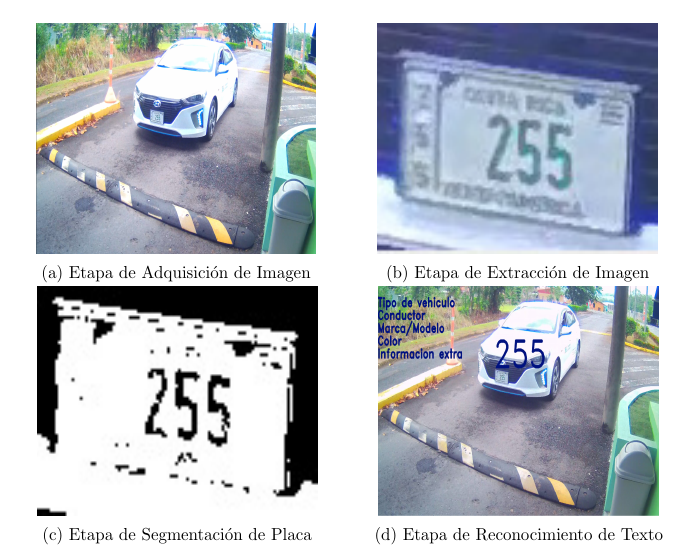
\includegraphics[width=0.8\linewidth]{fig/proy/ANPR_san_carlos.png}
	\caption{Etapas del ANPR.}
	\label{fig:anpr san carlos camara}
\end{figure}

Por el contrario, en la sede de San José, los vehículos ingresan rápidamente y no hay barreras que los detengan,
lo que reduce el tiempo disponible para la captura de imágenes. Además,
aunque se intentó reutilizar las cámaras existentes, estas no pueden ser reubicadas por motivos de seguridad.
Su ubicación actual--—en puntos elevados y con ángulos inclinados—--,
junto con condiciones de iluminación adversas (sol directo en las mañanas y escasa luz en las noches),
dificulta la visibilidad y complica el funcionamiento del sistema ANPR.
Aunque se usaron imágenes de placas costarricenses durante el entrenamiento,
estas fueron tomadas mayoritariamente en condiciones ideales: de día y en ángulos frontales,
lo que introdujo un sesgo en los datos.

Por estos motivos, el proyecto anterior no se llegó a implementar en ninguna de las dos sedes 
y actualmente se encuentra suspendido.

Dado que no se dispone de imágenes oficiales de las cámaras de seguridad ni de los equipos instalados
---por razones de seguridad institucional---, se ha optado por utilizar un croquis representativo para ilustrar 
la distribución aproximada de estos elementos dentro del campus. Esta representación no pretende ser un plano técnico,
sino una herramienta visual de apoyo que permite comprender mejor el contexto operativo 
en el que se desarrollará la solución propuesta.

\begin{figure}[H]
    \centering
    % Fila pacheco
    \begin{subfigure}[t]{0.45\textwidth}
        \centering
		\placeholderimage{0.3\textwidth}
        % \includegraphics[width=\linewidth]{fig/proy/example-image-pacheco_croquis_front}
        \caption*{Pacheco - Vista frontal}
    \end{subfigure}
    \hfill
    \begin{subfigure}[t]{0.45\textwidth}
        \centering
		\placeholderimage{0.3\textwidth}
        % \includegraphics[draft,width=\linewidth]{fig/proy/example-image-pacheco_croquis_up}
        \caption*{Pacheco - Vista superior}
    \end{subfigure}
    
	\vspace{1em}
	
	%Fila city
    \begin{subfigure}[t]{0.45\textwidth}
        \centering
		\placeholderimage{0.3\textwidth}
        % \includegraphics[draft,width=\linewidth]{fig/proy/example-image-city_croquis_front}
        \caption*{City - Vista frontal}
    \end{subfigure}
	\hfill
    \begin{subfigure}[t]{0.45\textwidth}
        \centering
		\placeholderimage{0.3\textwidth}
        % \includegraphics[draft,width=\linewidth]{fig/proy/example-image-city_croquis_up}
        \caption*{City - Vista superior}
    \end{subfigure}
	
	\vspace{1em}

    % Fila principal
    \begin{subfigure}[t]{0.45\textwidth}
        \centering
		\placeholderimage{0.3\textwidth}
        % \includegraphics[draft,width=\linewidth]{fig/proy/principal_croquis_front.png}
        \caption*{Principal - Vista frontal}
    \end{subfigure}
	\hfill
    \begin{subfigure}[t]{0.45\textwidth}
        \centering
		\placeholderimage{0.3\textwidth}
        % \includegraphics[draft,width=\linewidth]{fig/proy/principal_croquis_up.png}
        \caption*{Principal- Vista superior}
    \end{subfigure}
    \caption{Croquis de los sitios evaluados: Casa Pacheco, Estacionamiento City y Estacionamiento Principal.}
\end{figure}

\section{Retos en el control de acceso y disponibilidad de parqueos en el Campus San José}

El problema a solucionar es que el Campus Tecnológico Local San José del TEC presenta dificultades
para encontrar y acceder a espacios de estacionamiento, debido a la falta de coordinación entre
los distintos estacionamientos, la escasa visibilidad sobre su disponibilidad y la dependencia
de procedimientos manuales, lo que provoca molestias y pérdida de tiempo.

\section{Propuesta de un sistema de detección y reconocimiento de placas vehiculares}

En el Campus Tecnológico Local San José existen dificultades para encontrar
lugar de estacionamiento. Dada la descoordinación que existe entre los tres estacionamientos
de la universidad a los conductores se les dificulta encontrar con rapidez un lugar para estacionar.
Por ello se busca que las soluciones propuestas brinden al menos los siguientes requerimientos generales:

\begin{enumerate}
	\item Mejorar la gestión de espacios de estacionamiento en el Campus San José del TEC.
    \item Facilitar el acceso a información sobre disponibilidad de espacios.
	\item Usar recursos existentes cuando sea posible.
\end{enumerate}

Se espera entonces mejorar la fluidez de acceso a los estacionamientos brindando información a 
los conductores y guardas de seguridad para poder gestionar de forma más eficiente los estacionamientos,
facilitando encontrar lugar de estacionamiento y manteniendo orden en el lugar.
Asimismo, al aprovechar los recursos existentes, cámaras de video y computadoras, se puede brindar el 
prototipo de una solución de bajo costo para la institución.

En la propuesta de solución, que se brindará a continuación, se considerará la posibilidad de
extender la solución al Campus Tecnológico Local San Carlos.
Puesto que si bien el proyecto es solo para la Sede de San José, el Campus de San Carlos
ha manifestado el deseo de aplicar la solución también en dicha institución.

La propuesta en cuestión es el prototipo de un subsistema encargado de detección y 
reconocimiento de números de placas vehiculares (ANPR),
que será usado en un proyecto mayor de gestión inteligente de estacionamientos (IPLMS).
El sistema consta de cámaras instaladas en los accesos a los estacionamientos que envían los
datos capturados a un servidor local. Este servidor ejecutará un software IPLMS, que procesa la 
información en tiempo real. 
Los datos procesados son compartidos con dos salidas: una aplicación web,
donde los usuarios consultan la disponibilidad de espacios libres,
y un semáforo en la entrada de cada estacionamiento, que indica si existen espacios o no.

Dada la complejidad de un sistema completo de gestión de parqueos,
en este trabajo se aborda únicamente la etapa de reconocimiento automático de placas vehiculares (ANPR).
El subsistema ANPR consiste en aproximación mediante redes neuronales end-to-end. 

Los sistemas segmentados tradicionales presentan limitaciones:
dependen de conocer la cantidad de caracteres,
son sensibles a condiciones ambientales (iluminación, ángulo de visión, deformaciones),
y su desempeño está limitado por el “eslabón más débil” del pipeline, lo que dificulta su reajuste.

Una red end-to-end mitiga estos problemas al integrar todo el proceso de reconocimiento 
en una única arquitectura de aprendizaje profundo. Sin embargo, esto requiere grandes volúmenes 
de datos para entrenamiento \cite{endToEndDepthwise}. Para suplir esta carencia se desarrollará 
un generador de datos sintéticos de placas, que permita entrenar el modelo de reconocimiento de manera robusta.

La propuesta de solución se organiza en dos etapas principales: detección y reconocimiento, según los siguientes principios:

\begin{enumerate}

	\item \textbf{Captura de imágenes:}
Se emplean cámaras electrónicas instaladas en puntos estratégicos donde las placas sean visibles 
al ingreso de automóviles y motocicletas.


\item \textbf{Detección de placa:}  
      Se utiliza una red neuronal de detección de objetos para localizar y extraer la región correspondiente a la matrícula.  
      Existen múltiples modelos pre-entrenados que pueden adaptarse; en este caso se adopta **YOLOv11** 
		por su velocidad y precisión en tiempo real.  

\item \textbf{Reconocimiento de placa:}  
	A diferencia de los métodos basados en segmentación de caracteres, se emplea un modelo \textbf{end-to-end} 
		que integra la extracción y reconocimiento en una sola red convolucional.  
		Se consideran arquitecturas basadas en \textbf{CNN + CTC},
		entrenadas con datos sintéticos generados y posteriormente ajustadas con muestras reales.  

\end{enumerate}

\begin{figure}[H]
	\centering
	\placeholderimage{0.3\textwidth}
	% \includegraphics[width=\textwidth]{fig/proy/digrama-flujo-ANPR.jpg}
	\caption{Diagrama de flujo de sistema ANPR}
\end{figure}

\section{Objetivos del proyecto y organización del documento}

\textbf{Objetivo general: }

Desarrollar un prototipo de 
sistema automático para la detección y reconocimiento de caracteres en placas vehiculares costarricenses,
aplicando técnicas de visión por computadora y aprendizaje automático,
adaptado a las condiciones del Campus Local San José del Tecnológico de Costa Rica.

\textbf{Indicador:}
	\begin{enumerate}
		\item \textbf{Mejora relativa de desempeño frente al sistema base} \\
		\textbf{Descripción:} Comparación del desempeño general (en CAR, EMR, IoU) del sistema
		desarrollado frente a una solución base no entrenada localmente (ejemplo YOLOv8 + EasyOCR). \\
		\textbf{Unidad:} Porcentaje (\%) de mejora promedio en métricas clave. \\
		\textbf{Criterio de cumplimiento:} Mejora $\geq$ 5\%, con margen de tolerancia del $\pm 2$\% respecto a referencia. \\
		\textbf{Justificación:} Evalúa si el sistema propuesto aporta una mejora significativa frente
			solución genérica sin ajuste local. Al tratarse de un sistema orientado a condiciones específicas del campus,
			se espera una mejor de detección y reconocimiento. \\\\
	\end{enumerate}

\textbf{Objetivos específicos: }
\begin{enumerate}
	\item Preparar un conjunto de datos adecuado para el entrenamiento del sistema,
		combinando imágenes reales de placas vehiculares costarricenses con datos sintéticos generados por software.
		
		\textbf{Indicador}:
		\begin{enumerate}
			\item \textbf{Tamaño mínimo de dataset útil para entrenamiento}\\
			\textbf{Descripción:} Número de imágenes reales anotadas disponibles para entrenar el modelo \\
			\textbf{Unidad:} Imágenes \\
			\textbf{Criterio:} Se requiere obtener y etiquetar al menos 700 imágenes reales. \\
			\textbf{Criterio de cumplimiento:} Se cumple si el dataset base alcanza $\geq$ 700 imágenes reales etiquetadas. \\
			\textbf{Justificación:} Un volumen mínimo de datos reales es necesario para entrenar modelos
				de forma que aprenda característica de placas reales y no sobreajuste sobre datos sintéticos. \\ \\
		\end{enumerate}

		\textbf{Entregable}: Conjunto de datos etiquetado (mínimo 700 imágenes reales y datos sintéticos generados).

	\item Implementar técnicas de aumento de datos en tiempo real durante el entrenamiento para 
		robustecer el modelo ante condiciones adversas de iluminación, ángulo y resolución.

		\textbf{Indicadores:}
		\begin{enumerate}
			\item \textbf{Presencia de aumento de datos en el pipeline de entrenamiento} \\
			\textbf{Descripción:} 
			Verifica si se aplican transformaciones visuales en tiempo real en el conjunto de entrenamiento \\
			\textbf{Unidad:} Cumplimiento binario (Sí/No) \\
			\textbf{Criterio:}  El modelo aplica rotaciones, ruido, 
				distorsiones o transformaciones similares al menos en un 50\% de los datos. \\ 
			\textbf{Criterio de cumplimiento:} Si se verifica en código y entrenamiento que se aplican aumentos. \\
			\textbf{Justificación:} La aplicación de aumentos fortalece la capacidad del modelo
				para responder a variaciones reales en ángulo, iluminación y resolución,
				lo cual es especialmente importante en ambientes no controlados \\

			\item \textbf{Variación de desempeño con y sin aumento de datos} \\
			\textbf{Descripción: }Evalúa si el modelo entrenado con aumento presenta mayor robustez frente a perturbaciones \\
			\textbf{Unidad: }Diferencia porcentual de CAR / EMR \\
			\textbf{Criterio: }La caída de precisión ante perturbaciones debe ser menor 
			en el modelo con aumento que en uno sin aumento. \\
			\textbf{Criterio de cumplimiento:} Si $\Delta$ caída es menor o igual al $\leq$ 5\%
				frente a perturbaciones comparado con baseline sin aumento. \\
			\textbf{Justificación}:  Este indicador permite comprobar que los aumentos de datos no solo están presentes,
				sino que realmente aportan robustez y hacen al sistema menos sensible a perturbaciones\\ \\
		\end{enumerate}

		\textbf{Entregables}: Módulo o script configurado de aumento de datos integrado al pipeline de entrenamiento

	\item Diseñar y entrenar una arquitectura de reconocimiento automático de placas basada en una red neuronal convolucional 
		moderna (end-to-end), que incluya una etapa de detección de región de placa 
		y otra de reconocimiento de texto sin segmentación manual.

		\textbf{Indicador}:
		\begin{enumerate}
			\item \textbf{Tipo de arquitectura desarrollada} \\
			\textbf{Descripción: }Características que debe poseer la arquitectura diseñada de detección
				y reconocimiento de placa. \\
				\textbf{Unidad: }Binario (Si/No). \\
			\textbf{Criterio: }Arquitectura no segmentada + entrada imagen con salida texto. \\
			\textbf{Criterio de cumplimiento:} El sistema presenta bloques claramente identificados \\
				(detección, reconocimiento, entrada imagen y salida de texto). \\
			\textbf{Justificación:}  Asegura que el sistema sea moderno y capaz
				de reconocer placas completas sin necesidad de separar caracteres manualmente \\\\
		\end{enumerate}

		\textbf{Entregables:} Modelos entrenados y listos para inferencia (detección y reconocimiento).

	\item Evaluar el desempeño del sistema propuesto comparándolo contra un modelo base
		mediante métricas de reconocimiento y detección, con el fin de validar mejoras en precisión,
		exactitud completa y robustez.

		\begin{enumerate}
			\item \textbf{Tasa de reconocimiento de caracteres (Character Accuracy Rate, CAR)} \\
				\textbf{Descripción:} Mide la proporción de caracteres correctamente reconocidos por el modelo. \\
				\textbf{Unidad:} Porcentaje (\%) \\
				\textbf{Criterio de evaluación:} 
					Se considera aceptable si el modelo es mejora respecto de la línea base. \\
				\textbf{Criterio de cumplimiento:} Mejora$\geq 5\%$. \\
				\textbf{Justificación:}  El CAR mide la capacidad del sistema para reconocer caracteres individuales
				correctamente. Es una métrica central para evaluar la precisión del reconocimiento parcial de placas,
				especialmente útil cuando algunas predicciones son parcialmente correctas. \\
			\item \textbf{Error de secuencia completa (Exact Match Rate)} \\
				\textbf{Descripción:}
				Proporción de placas en las que se predice correctamente la secuencia completa de caracteres. \\
				\textbf{Unidad:} Porcentaje (\%) \\
				\textbf{Criterio:} Mejora la capacidad de reconocimiento total entre la secuencia predicha y la real. \\
				\textbf{Criterio de cumplimiento:} Mejora$\geq 10\%$ \\
				\textbf{Justificación:}  El EMR evalúa la proporción de placas completamente reconocidas sin errores.
				Esta métrica representa un caso ideal de éxito y es crítica para determinar si el sistema 
				puede ser usado en contextos donde los errores de una letra o número no son tolerables. \\
			\item mIoU (Mean Intersection over Union) en detección de placas \\
				\textbf{Descripción:} Evalúa qué tan bien se detecta la región de la placa en relación con la anotación real. \\
				\textbf{Unidad:} Valor entre 0 y 1 \\
				\textbf{Criterio:} Se considera aceptable si detecta mejor la placa respecto al modelo base. \\
				\textbf{Criterio de cumplimiento:} Mejora$\geq0.03$ \\
				\textbf{Justificación}:  mIoU mide qué tan bien el sistema detecta la región de la placa.
				Esta métrica es esencial para garantizar que el texto reconocido provenga de la región correcta
				de la imagen y no se contamine con información visual irrelevante.\\ \\
		\end{enumerate}

		\textbf{Entregables:} Documentación y reporte técnico de resultados de las evaluaciones.
\end{enumerate}

En cuanto a la estructura, este documento se organiza de la siguiente manera:
\begin{itemize}
    \item El \textbf{Capítulo 1} presenta la introducción, incluyendo el contexto, 
		antecedentes, el problema, un esbozo de la solución y los objetivos.
    \item El \textbf{Capítulo 2} expone el marco teórico y el estado del arte en sistemas
		de reconocimiento de placas y gestión de estacionamientos inteligentes.
    \item El \textbf{Capítulo 3} describe la metodología empleada para el desarrollo de la solución.
    \item El \textbf{Capítulo 4} detalla los resultados obtenidos y el análisis de desempeño del sistema.
    \item Finalmente, el \textbf{Capítulo 5} presenta las conclusiones y recomendaciones para trabajos futuros.
\end{itemize}


\section{Sistema de almacenamiento energético}

Después de las secciones anteriores ya ha guiado al lector hasta este
punto en donde solo resta presentar una propuesta general de solución
del problema técnico concreto.

Para aclarar la solución se hace uso de un diagrama de bloques (ver
\figref{fig:diagbloques}) o diagrama de flujo general, es decir,
desde un nivel de abstracción muy alto, donde no sea necesario entrar
en detalles técnicos, porque aún no han sido expuestos.

